\section{Lezione del 25 novembre}
\subsection{Situazioni fondamentali}
Nella lezione precedente abbiamo visto la sequenza, definita come un $c[e_1 > \land \neg c[e_2 \land c[e_1e_2$ che mostrava anche il fatto di avere una relazione di \textbf{dipendenza causale} tra $e_1$ ed $e_2$.

\subsubsection{Concorrenza}
Sia $\Sigma = (B,E,F, c_{in})$ un sistema elementare con $c \in C_{\Sigma};\ e_1,e_2 \in E$. Diciamo che i due eventi sono concorrenti in un caso $c$, se e solo se $c[\{e_1e_2\} >$. \\

\begin{center}
    \begin{tikzpicture}[node distance=2.3cm,>=stealth',bend angle=45,auto]
        \tikzstyle{place}=[circle,thick,draw=blue!75,fill=blue!20,minimum size=6mm]
        \tikzstyle{transition}=[rectangle,thick,draw=blue!75,minimum size=4mm]
        
        \node [place, tokens=1] (p1)     {}; %P1
        \node [transition] (p13) [right of=p1, label=above:$e_2$] {}                   %this is new p
            edge [pre]  (p1);
        \node [place] (p3) [right of=p13]   {} %P1
            edge [pre] (p13);
            
        \node [place, tokens=1] (p2) [below of=p1]   {}; %P1
        \node [transition] (p24) [right of=p2, label=above:$e_1$] {}                   %this is new p
            edge [pre]  (p2);
        \node [place] (p4) [right of=p24]   {}
            edge [pre]  (p24);%P1
        \node [transition] (p24p13) [above right of=p4] {}                   %this is new p
            edge [pre]  (p4)
            edge [pre]  (p3);
        \node [place] (p5) [right of = p24p13] {}
            edge [pre]  (p24p13);
    \end{tikzpicture}
\end{center}

Quindi abbiamo due eventi che sono indipendenti, che non hanno quindi pre e post condizioni/ che interferiscono, e che sono abilitati in $c$. E quindi i due eventi possono occorrere in un unico passo.

\subsubsection{Conflitto}
Sia $\Sigma = (B,E,F, c_{in})$ un sistema elementare con $c \in C_{\Sigma};\ e_1,e_2 \in E$. Diciamo che i due eventi sono in conflitto in un caso $c$, se e solo se $c[e_1> \land \ c[e_2> \land \neg c[\{e_1e_2\} > $. \\

In poche parole in questo caso abbiamo che entrambi sono abilitati, come nella concorrenza, ma l'occorrenza di uno disabilita l'altro.


\begin{figure}[H]
\centering
\begin{subfigure}{.5\textwidth}
  \begin{center}
    \begin{tikzpicture}[node distance=1.3cm,>=stealth',bend angle=45,auto]
        \tikzstyle{place}=[circle,thick,draw=blue!75,fill=blue!20,minimum size=6mm]
        \tikzstyle{transition}=[rectangle,thick,draw=blue!75,minimum size=4mm]
        
        \node [place, tokens=1] (p1)     {}; %P1
        \node [transition] (p11) [below left of=p1, label=left:$e_1$] {}                   %this is new p
            edge [pre]  (p1);
        \node [transition] (p12) [below right of=p1, label=right:$e_2$] {}                   %this is new p
            edge [pre]  (p1);
            
        \node [place] (p123) [below of=p12]   {} %P1
            edge [pre] (p12);
        \node [place] (p113) [below of=p11]   {} %P1
            edge [pre] (p11);
    \end{tikzpicture}
    \caption{in avanti: forward}
\end{center}
\end{subfigure}%
\begin{subfigure}{.5\textwidth}
\begin{center}
    \begin{tikzpicture}[node distance=1.3cm,>=stealth',bend angle=45,auto]
        \tikzstyle{place}=[circle,thick,draw=blue!75,fill=blue!20,minimum size=6mm]
        \tikzstyle{transition}=[rectangle,thick,draw=blue!75,minimum size=4mm]
        
        \node [place, tokens=1] (p1)     {}; %P1
        \node [place, tokens=1] (p2)  [left of=p1]   {}; %P1
        \node [transition] (p11) [below of=p1, label=right:$e_2$] {}                   %this is new p
            edge [pre]  (p1);
        \node [transition] (p12) [below of=p2, label=left:$e_1$] {}                   %this is new p
            edge [pre]  (p2);
        \node [place] (p123) [below right of=p12]   {} %P1
            edge [pre] (p11)
            edge [pre] (p12);
    \end{tikzpicture}
    \caption{all'indietro: backward}
\end{center}
\end{subfigure}%
\end{figure}

In questi tipi di conflitti, modelli, non viene specificato quele dei due eventi scatterà. Sappiamo solamente che se uno dei due scatta, l'altra avrà delle post condizioni vere che non gli permettono di scattare. 

Nel caso in cui prendiamo una possibile configurazione successiva, ad esempio ci ritroviamo:
\begin{figure}[H]
\centering
\begin{subfigure}{.5\textwidth}
  \begin{center}
    \begin{tikzpicture}[node distance=1.3cm,>=stealth',bend angle=45,auto]
        \tikzstyle{place}=[circle,thick,draw=blue!75,fill=blue!20,minimum size=6mm]
        \tikzstyle{transition}=[rectangle,thick,draw=blue!75,minimum size=4mm]
        
        \node [place] (p1)     {}; %P1
        \node [transition] (p11) [below left of=p1, label=left:$e_1$] {}                   %this is new p
            edge [pre]  (p1);
        \node [transition] (p12) [below right of=p1, label=right:$e_2$] {}                   %this is new p
            edge [pre]  (p1);
            
        \node [place ] (p123) [below of=p12]   {} %P1
            edge [pre] (p12);
        \node [place, tokens=1] (p113) [below of=p11]   {} %P1
            edge [pre] (p11);
    \end{tikzpicture}
    \caption{in avanti: forward}
\end{center}
\end{subfigure}%
\begin{subfigure}{.5\textwidth}
\begin{center}
    \begin{tikzpicture}[node distance=1.3cm,>=stealth',bend angle=45,auto]
        \tikzstyle{place}=[circle,thick,draw=blue!75,fill=blue!20,minimum size=6mm]
        \tikzstyle{transition}=[rectangle,thick,draw=blue!75,minimum size=4mm]
        
        \node [place] (p1)     {}; %P1
        \node [place] (p2)  [left of=p1]   {}; %P1
        \node [transition] (p11) [below of=p1, label=right:$e_2$] {}                   %this is new p
            edge [pre]  (p1);
        \node [transition] (p12) [below of=p2, label=left:$e_1$] {}                   %this is new p
            edge [pre]  (p2);
        \node [place , tokens=1] (p123 ) [below right of=p12]   {} %P1
            edge [pre] (p11)
            edge [pre] (p12);
    \end{tikzpicture}
    \caption{all'indietro: backward}
\end{center}
\end{subfigure}%
\end{figure}


Ci chiediamo che cosa sia successo al nostro sistema. Ovvero conoscere che cosa ha portato il sistema nella situazione attuale. \\

Nella figura [(a)] sappiamo che è scattato l'evento $e_1$, quindi qualcosa avrà azionato $e_1$ riportando ulteriori informazioni, invece nella figura [(b)] abbiamo che è vera la post condizioni di entrambi gli eventi e quindi possiamo dire che è scattato uno dei due eventi senza precisamente sapere quale. Questo lo riconosciamo perché nella configurazione precedente era vera sola una delle due, quindi era vera o solo la pre di $e_1$ o solo quella di $e_2$. 

\subsubsection{Confusione}
Il conflitto e la concorrenza interferiscono l'una con l'altra generando confusione. Si hanno principalmente due casi di confusione:
\begin{enumerate}
    \item Il primo caso è una confusione \textbf{asimmetrica}. Consideriamo il fatto che possono scattare contemporaneamente due eventi.
    Nel nostro caso abbiamo gli eventi $e_1$ e $e_2$ che possono scattare in maniera concorrente. Lo scatto mi porta nel nuovo caso $b_4$, $b_5$.
    \begin{center}
        \begin{tikzpicture}[node distance=1.3cm,>=stealth',bend angle=45,auto]
            \tikzstyle{place}=[circle,thick,draw=blue!75,fill=blue!20,minimum size=6mm]
            \tikzstyle{transition}=[rectangle,thick,draw=blue!75,minimum size=4mm]
            
            \node [place, tokens=1] (b2) [label=right:$b_2$]    {}; %P1
            \node [transition] (e2) [below of=b2, label=right:$e_2$] {}                   %this is new p
                edge [pre]  (b2);
            \node [place] (b4) [below of=e2, label=right:$b_4$]    {} %P1
                edge [pre]  (e2);
            \node [place, tokens = 1] (b3) [left of=b4, label=above:$b_3$]    {}; %P1
            \node [place, tokens = 1] (b1) [left of=b3, label=above:$b_1$]    {}; %P1  
            \node [transition] (b1b3) [below right of=b1, label=left:$e_1$] {}                   %this is new p
                edge [pre]  (b1)
                edge [pre]  (b3);
            \node [transition] (b3b4) [below right of=b3, label=right:$e_3$] {}                   %this is new p
                edge [pre]  (b3)
                edge [pre]  (b4);
            \node [place] (p123) [below of=b3b4,label=right:$b_6$]   {} %P1
                edge [pre] (b3b4);
             \node [place] (p123) [below of=b1b3,label=left:$b_5$]   {} %P1
                edge [pre] (b1b3);
        \end{tikzpicture}
    \end{center}
    Se questi vengono eseguiti nello stesso passo, nell'esecuzione di $c[\{e_1e_2\} > c'$ è stato risolto un conflitto? Teniamo conto del fatto che $c = \{b_1,b_2,b_3\} $ e $c = \{b_4,b_5\}$. Non sapendo quale sia stato l'ordine delle due non possiamo stabilire se sia o meno stato risolto un conflitto. \\
    Questo ci porta ad avere due possibilità, entrmabe ammisibili:
    \begin{itemize}
        \item occorre prima $e_1$ senza essere in conflitto 
        \item occorre prima $e_2$ e poi il conflitto tra $e_1$ e $e_3$ viene risolto a favore di $e_1$
    \end{itemize}
    \item Il secondo caso è una confusione \textbf{simmetrica}. Consideriamo il fatto che abbiamo due eventi entrambi abilitati e i due possono occorrere contemporaneamente.
    Nel nostro caso abbiamo gli eventi $e_1$ e $e_3$ che possono occorrere in maniera concorrente. Passando dallo stato $b_1$, $_2$ allo stato $b_3$, $_5$
    \begin{center}
        \begin{tikzpicture}[node distance=1.3cm,>=stealth',bend angle=45,auto]
            \tikzstyle{place}=[circle,thick,draw=blue!75,fill=blue!20,minimum size=6mm]
            \tikzstyle{transition}=[rectangle,thick,draw=blue!75,minimum size=4mm]
            
            \node [place, tokens=1] (b2) [label=left:$b_2$]    {}; %P1
            \node [transition] (e2) [below left of=b2, label=right:$e_2$] {}                   %this is new p
                edge [pre]  (b2);
            \node [transition] (e3) [below right of=b2, label=right:$e_3$] {}                   %this is new p
                edge [pre]  (b2);   
            \node [place, tokens=1] (b1) [above left of= e2, label=left:$b_1$]    {} %P1
                edge [post]  (e2);
                
           \node [transition] (e1) [below left of=b1, label=left:$e_1$] {}                   %this is new p
                edge [pre]  (b1);
                
             \node [place] (b3) [below of = e1, label=left:$b_3$]    {} %P1
                edge [pre]  (e1); 
            \node [place] (b4) [below of= e2, label=left:$b_4$]    {} %P1
                edge [pre]  (e2); 
            \node [place] (b5) [below of= e3, label=left:$b_5$]    {} %P1
                edge [pre]  (e3);
        \end{tikzpicture}
    \end{center}
    
    Se scatta $e_1$ il conflitto tra $e_1$ e $e_2$ viene risolto a favore di $e_1$, a questo punto resta solamente $e_3$ abilitato, e quindi scatta.\\
    Se scatta $e_3$ il conflitto tra $e_3$ e $e_2$ viene risolto a favore di $e_3$, a questo punto resta solamente $e_1$ abilitato, e quindi scatta.\\
    Questo comporta che nell'esecuzione di $c[\{e_1e_3\} > c'$ non è possibile stabilire se è stato risolto un conflitto tra $e_1$ ed $e_2$ oppure tra $e_2$ ed $e_3$.\\
    Non è pertanto precisamente specificato chi ha deciso, o chi ha la responsabilità di stabilire chi scatta. 
\end{enumerate} 

\subsection{Sottorete}
Siano $N=(B,E,F)$ e $N_1=(B_1,E_1,F_1)$ due reti elementari. Si dice che $N_1$ è \textbf{sottorete} di $N$  se e solo se: 
\begin{itemize} 
    \item $B_1\subseteq B$, quindi l'insieme delle condizioni della rete $N_1$ è sottoinsieme di quello della rete $N$ 
    \item $E_1\subseteq E$, quindi l'insieme degli eventi della rete $N_1$ è sottoinsieme di quello della rete $N$ 
    \item $F_1=F\cap[(B_1\times E_1)\cup (E_1\times B_1)]$, ovvero la relazione di flusso di $N_1$ è definita come la restrizione della relazione di flusso di $N$ rispetto alle condizioni e $B_1$ e agli eventi $E_1$ (tengo quindi solo gli archi di $N$ che connettono eventi e condizioni di $N_1$) 
\end{itemize}

Esiste inoltre la \textbf{sottorete generata da condizioni}.\\
Si dice che $N_1$ è \textbf{sottorete generata da} $B_1$ di $N$ (ovvero di sottorete generata da un insieme di condizioni)  se e solo se: 
\begin{itemize}
    \item $B_1\subseteq B$, quindi l'insieme delle condizioni della rete $N_1$ è sottoinsieme di quello della rete $N$ 
    \item $E_1=  ^\bullet B_1\cup B_1^\bullet$, ovvero come eventi si hanno tutti quegli eventi che sono collegati in $N$ alle condizioni incluse nell'insieme di condizioni $B_1$, prendendo quindi tutti i pre-eventi e i post-eventi delle condizioni dell'insieme $B_1$ 
    \item $F_1=F\cap[(B_1\times E_1)\cup (E_1\times B_1)]$, ovvero la relazione di flusso di $N_1$ è definita come la restrizione della relazione di flusso di $N$ rispetto alle condizioni $B_1$ e agli eventi $E_1$ 
\end{itemize} 
Non ho quindi una sottorete generata da un insieme arbitrario di condizioni ed eventi ma questi ultimi sono direttamente presi in relazione all'insieme delle condizioni scelto.\\

Esiste inoltre la \textbf{sottorete generata da eventi}.\\
Siano $N=(B,E,F)$ e $N_1=(B_1,E_1,F_1)$ due reti elementari.\\ 
Si dice che $N_1$ è \textbf{sottorete generata da} $E_1$ di $N$ (ovvero di sottorete generata da un insieme di eventi)  se e solo se: 
\begin{itemize} 
    \item $B_1= ^\bullet E_1\cup E_1^\bullet$, ovvero come condizioni si hanno tutte quelle condizioni che sono collegati in $N$ agli eventi inclusi nell'insieme di eventi $E_1$, prendendo quindi tutte e precondizioni e le postcondizioni degli eventi dell'insieme $E_1$ 
    \item $E_1\subseteq E$, quindi l'insieme degli eventi della rete $N_1$ è sottoinsieme di quello della rete $N$ 
    \item $F_1=F\cap[(B_1\times E_1)\cup (E_1\times B_1)]$, ovvero la relazione di flusso di $N_1$ è definita come la restrizione della relazione di flusso di $N$ rispetto alle condizioni $B_1$ e agli eventi $E_1$ 
\end{itemize} 
Non ho quindi una sottorete generata da un insieme arbitrario di condizioni ed eventi ma le prime sono direttamente prese in relazione all'insieme degli eventi scelto

\subsection{Operazioni di Composizione per Reti di Petri}
Data una rete $N=(B,E,F,c_0)$ questa può essere ottenuta componendo altre reti di Petri. Si hanno in letteratura 3 modi principali:
\begin{enumerate}
    \item la \textbf{composizione sincrona}
    \begin{figure}[H]
\centering
\begin{subfigure}{.5\textwidth}
  \begin{center}
   \begin{tikzpicture}[node distance=1.3cm,>=stealth',bend angle=45,auto]
        \tikzstyle{place}=[circle,thick,draw=blue!75,fill=blue!20,minimum size=6mm]
        \tikzstyle{transition}=[rectangle,thick,draw=blue!75,minimum size=4mm]
        
        \node [place, tokens=1] (b2) [label=above left:$N_1$]    {}; %P1
        \node [transition,fill=yellow!50 ] (e2) [below of=b2, label=right:\mbox{send}] {}                   %this is new p
            edge [pre]  (b2);
        \node [place] (b1) [below of= e2]    {} %P1
            edge [pre]  (e2);
        \node [transition] (e1) [below of=b1] {}                   %this is new p
            edge [pre]  (b1);
        \node [place] (b3) [left of = e1]    {} %P1
            edge [pre]  (e1); 
        \node [transition] (b4) [left of= e2]    {} %P1
            edge [pre]  (b3)
            edge [post] (b2); 
    \end{tikzpicture}
\end{center}
\end{subfigure}%
\begin{subfigure}{.5\textwidth}
\begin{center}
     \begin{tikzpicture}[node distance=1.3cm,>=stealth',bend angle=45,auto]
        \tikzstyle{place}=[circle,thick,draw=red!75,fill=red!20,minimum size=6mm]
        \tikzstyle{transition}=[rectangle,thick,draw=red!75,minimum size=4mm]
        
        \node [place, tokens=1] (b2) [label=above left:$N_1$]    {}; %P1
        \node [transition,fill=yellow!50 ] (e2) [below of=b2, label=left:\mbox{recieve}] {}                   %this is new p
            edge [pre]  (b2);
        \node [place] (b1) [below of= e2]    {} %P1
            edge [pre]  (e2);
        \node [transition] (e1) [below of=b1] {}                   %this is new p
            edge [pre]  (b1);
        \node [place] (b3) [right of = e1]    {} %P1
            edge [pre]  (e1); 
        \node [transition] (b4) [right of= e2]    {} %P1
            edge [pre]  (b3)
            edge [post] (b2); 
    \end{tikzpicture}
\end{center}
\end{subfigure}%
\end{figure}
    Portandoci ad ottenere, quando vogliamo unire i due campi, la seguente rete:
    \begin{figure}[H]
        \centering
        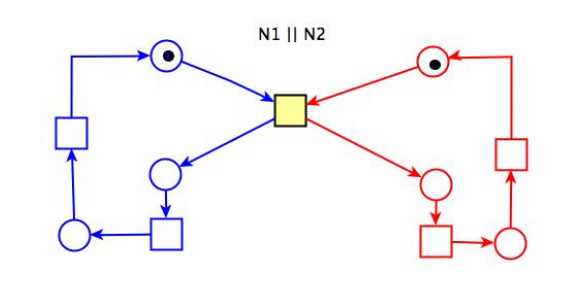
\includegraphics[scale=.5]{IMM/sincro.PNG}
    \end{figure}
     Lo scatto dell'evento, in maniera sincrona, rende vere le postcondizioni nelle due componenti e false le due precondizioni.\\
    \item la \textbf{composizione asincrona}
    Supponiamo di avere i modelli di due componenti, $N_1$, che invia in un canale un messaggio (per esempio in un buffer), e $N_2$, che riceverà il messaggio solo quando esso sarà disponibile:
    \begin{figure}[H]
        \centering
        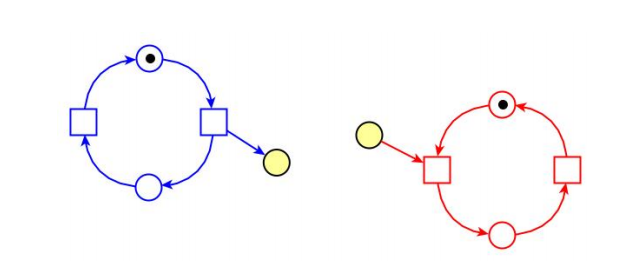
\includegraphics[scale=.5]{IMM/comp_asi.PNG}
    \end{figure}
    In questo caso, a differenza dell'esempio precedente, non identifichiamo eventi ma condizioni. Identifico quindi il canale (le due condizioni) come uno solo, che avrà il pre-evento in una componente e il post-evento nell'altra.\\ 
    Quindi il pre-evento, nella componente $N_1$, può scattare solo se questa nuova condizione condivisa è libera, indipendentemente dalla componente $N_2$. L'evento in $N_2$ può scattare solo se la condizione condivisa è marcata, indipendentemente dallo stato della prima componente, liberando il canale di comunicazione.\\
    \begin{figure}[H]
        \centering
        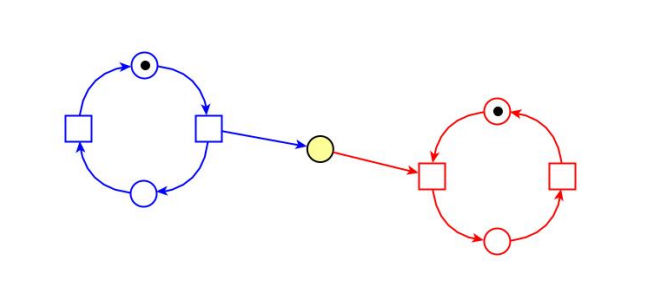
\includegraphics[scale=.5]{IMM/comp_asi2.PNG}
    \end{figure}
    \item la \textbf{composizione mista, tra sincrona e asincrona}
\end{enumerate}

\subsection{Processi non sequenziali}
Parliamo ora di sistemi non sequenziali, ad ordini parziali.\\ 
Definiamo $N=(B,E,F)$ come una \textbf{rete causale}, detta anche rete di occorrenze senza conflitti, se e solo se:
\begin{itemize}
    \item $\forall b\in B:|^{\bullet}b|\leq 1\land |b^{\bullet}|\leq 1$, ovvero non si hanno conflitti, quindi per ogni condizione si ha al più un pre evento e un post evento (avendo quindi al più un arco entrante e al più uno uscente)
    \item $\forall x,y\in B\cup E:(x,y)\in F^+\implies (y,x)\not\in F^+$, ovvero non si hanno cicli, quindi presi due elementi collegati da una sequenza di archi orientati, avendo un cammino tra i due elementi ($F^+$ è la chiusura transitiva della relazione $F$) non ho anche un cammino opposto tra i due
    \item $\forall e\in E:\{x\in B\cup E| xF^*e\}$ è finito, ovvero si ha un numero finito di pre-elementi di un certo elemento
\end{itemize}

Sono quindi reti che registrano un comportamento e quindi non si hanno conflitti (che in caso sono sciolti registrando solo quello che è effettivamente successo e non quello che potrebbe succedere). Si registra una run del sistema. Non si hanno nemmeno cicli perché ogni ripetizione dell'evento viene concatenata a quella prima (come detto nell'esempio dopo le righe tratteggiate in viola si cominciava da capo).\\ 
 
Ad una rete causale è possibile associare un ordine parziale: $(X,\leq)=(B\cup E, F^*)$. Questo ci dice che un elemento è minore di un altro se esiste un cammino orientato dall'uno all'altro (si specifica che $F^*$ non mi farà mai identificare $x$ con $x$, non ci sarà mai un camino su se stesso).

\subsubsection{Relazioni}
Data una rete causale $N=(B,E,F)$ e dato un ordine parziale $(X, \leq)$ con $X=B\cup E$ si ha che si può interpretare la relazione d'ordine come indipendenza o dipendenza causale.
Siano presi $x,y\in X$ come elementi che occorrono nella storia di $X=B\cup E$ si hanno le seguenti diciture: 
\begin{itemize} 
    \item $x\leq y$ (avendo un cammino da $x$ a $y$) corrisponde a \textbf{$x$ causa $y$}, ovvero si ha una relazione di dipendenza causale tra i due 
    \item $x \mbox{ \textbf{li} }y$ indica che $x\leq y\lor y\leq x$ e quindi corrisponde a \textbf{$x$ e $y$ sono casualmente dipendenti}. Si ha che \textbf{li} può venire letto come \textit{linea} ($x$ in linea con $y$) avendo che uno dei due precede l'altro 
    \item $x \mbox{ \textbf{co} }y$ indica che $\neg(x< y)\land \neg(y < x)$ e quindi corrisponde a \textbf{$x$ e $y$ sono casualmente indipendenti}, avendo che i due elementi non si precedono a vicenda, non sono ordinati. \textbf{co} sta per \textit{concurrency} 
\end{itemize}

\textbf{Line} (li), \textbf{Concurrency} (co) hanno alcune proprietà: sono entrambe simmetriche,\textbf{non} transitive e sono riflessive.

Data una rete causale $N=(B,E,F)$ e dato un ordine parziale $(X, \leq)$ con $X=B\cup E$ definiamo: $C\subseteq X$ come:
\begin{itemize}
    \item \textbf{co-set}  se e solo se $\forall x,y\in C:  x\mbox{ \textbf{co }}y$, quindi $C$ è una clique della relazione \textbf{co}
    \item \textbf{taglio}  se e solo se $C$ è un co-set massimale (tutti gli elementi nel taglio sono in relazione \textbf{co})
\end{itemize}

Definiamo $C$ come co-set massimale  se e solo se $\forall y\in X \land y \notin C$ si ha che: $\exists c\in C: y \mbox{ non è il relazione \textbf{co}  con } c$. Quindi in $C$ definito o come \textbf{co-set} o come \textbf{taglio} si ha che vale la transitività.\\
  
Definiamo: $L\subseteq X$ come:
\begin{itemize}
    \item \textbf{li-set}  se e solo se $\forall x,y\in L:  x\mbox{ \textbf{li }}y$
    \item \textbf{linea}  se e solo se $L$ è un li-set massimale
\end{itemize}

Alcune note:
\begin{itemize}
    \item in un \textbf{co-set} la relazione \textbf{co} è transitiva
    \item in un \textbf{li-set} la relazione \textbf{li} è transitiva.
\end{itemize}
Tagli e linee possono essere fatti sia di condizioni che di eventi.